%% Supplementary material for "DASH: Bounded-State Execution for Low-Latency
%% Streaming Machine Learning with Externalised State" (revision v4).
\documentclass[10pt,a4paper]{article}
\usepackage[margin=2.2cm]{geometry}
\usepackage{amsmath,amssymb}
\usepackage{booktabs,tabularx,array,multirow,longtable}
\usepackage{graphicx}
\usepackage{xurl}
\usepackage[hidelinks]{hyperref}
\graphicspath{{figures/}}
\newcolumntype{Y}{>{\raggedright\arraybackslash}X}
\renewcommand{\thesection}{S\arabic{section}}
\renewcommand{\thetable}{S\arabic{table}}
\renewcommand{\thefigure}{S\arabic{figure}}
\renewcommand{\theequation}{S\arabic{equation}}
\setlength{\parskip}{3pt}

\title{Supplementary Material\\[4pt]\large DASH: Bounded-State Execution for Low-Latency Streaming Machine Learning with Externalised State}
\author{Seonwoo Kim \and V. L. Raju Chinthalapati}
\date{Revision v4}

\begin{document}
\maketitle

\noindent This supplement accompanies the main paper. Sections S1--S5 give definitions, provenance details and repeat-level values for the evidence used in the paper; every measured value in them was recomputed from raw records during the revision (Section~\ref{sec:repro}); values copied from artefacts or code (Table~\ref{tab:thr}, hyperparameters) are identified as such. Section~\ref{sec:breadth} retains the historical summaries of the earlier evaluation of a previous implementation with an explicit provenance status: they were \emph{not} recomputed and are not evidence for any claim in the paper. Section~\ref{sec:repro} documents hashes, commands and the mapping from records to tables and figures. Latencies are in milliseconds unless a table states microseconds.

%% ------------------------------------------------------------------
\section{Feature and label definitions}
\label{sec:features}
For stream $k$, let $\mathcal{L}_t$ be the trades with timestamps in second $[t,t+1)$, each with price $p_i$, quantity $q_i$ and aggressor side $s_i\in\{+1,-1\}$ (buyer- or seller-initiated, from the exchange's maker flag). Seconds without trades produce no row, so $t$ indexes populated rows. Per row,
\begin{align}
V_t &= \textstyle\sum_{i\in\mathcal{L}_t} q_i, \qquad C_t=|\mathcal{L}_t|, \qquad \mathrm{VWAP}_t=\frac{\sum_{i} p_i q_i}{\sum_i q_i},\qquad r_t=\log\frac{\mathrm{VWAP}_t}{\mathrm{VWAP}_{t-1}},\\
v_t &= \lambda v_{t-1}+(1-\lambda)r_t^2,\quad v_1=r_1^2,\qquad \hat\sigma_t=\sqrt{v_t+\epsilon},\qquad \lambda=0.94,\ \epsilon=10^{-9},\\
\mathrm{OFI}_t &= Q_{t,\mathrm{buy}}-Q_{t,\mathrm{sell}},\qquad \mathrm{Imb}_t=\frac{Q_{t,\mathrm{buy}}-Q_{t,\mathrm{sell}}}{Q_{t,\mathrm{buy}}+Q_{t,\mathrm{sell}}+\epsilon},\qquad \mathrm{VolSpike}_t=\frac{V_t}{\bar V_t+\epsilon},
\end{align}
where $Q_{t,\mathrm{buy}}$ and $Q_{t,\mathrm{sell}}$ are the buyer- and seller-initiated volumes and $\bar V_t$ is the mean volume of the last $W_{\mathrm{vol}}=60$ populated rows (generator option \texttt{--vol-spike-win}, default 60). The feature vector is $X_t=[r_t,\hat\sigma_t,\mathrm{OFI}_t,\mathrm{Imb}_t,\mathrm{VolSpike}_t,C_t]$, stored as float32 in the order recorded in the scaler artefact: \texttt{r\_t, sigma\_hat, OFI\_t, Imbalance\_t, VolSpike\_t, msg\_count}. All features use rows up to and including $t$. The benchmarks replay these precomputed rows; feature generation is not timed.

The label uses $R^{(H)}_t=\sum_{i=1}^{H}r_{t+i}$ with $H=30$ populated rows (implemented as a cumulative-sum difference over $r_{t+1},\dots,r_{t+H}$); rows whose forward window is incomplete (the last $H$ rows) are dropped. $y_t=2$ if $R^{(H)}_t\ge\alpha\sqrt{H}\hat\sigma_t$, $y_t=1$ if $R^{(H)}_t\le-\alpha\sqrt{H}\hat\sigma_t$, and $y_t=0$ otherwise, with $\alpha=2$. Because $H$ counts populated rows, the horizon equals 30 seconds only without empty seconds. Causal feature carry-over across a split boundary (features at $t$ use earlier rows) is distinct from future-label leakage (labels at $t$ use later rows); only the latter is addressed by the training gap below.

%% ------------------------------------------------------------------
\section{Training protocol, thresholds and the threshold-selection defect}
\label{sec:training}
\paragraph{What the archived code implements (status: code only).} At the pinned commit, \texttt{train\_2.py} sorts rows by time, sets \texttt{split = int(n*(1-val\_ratio))} with default \texttt{val\_ratio=0.2}, uses rows \texttt{[0, split-gap)} for training and \texttt{[split, n)} for validation with default \texttt{gap=H=30} rows, fits the z-score mean and standard deviation on the training rows only, and trains Stage~1 (shock versus normal) on all training rows and Stage~2 (positive versus negative) on training rows with a true shock. Hyperparameters in the code: XGBoost Stage~1 with 2,000 trees, depth 3, learning rate 0.03, \texttt{scale\_pos\_weight} from the training class ratio, seed 100, no early stopping; XGBoost Stage~2 with up to 2,500 trees, depth 3, seed 42 and early stopping after 80 rounds \emph{on the validation shock rows}; random forests with 10 trees, depth 4, minimum leaf size 20, balanced class weights, seeds 52 and 53; logistic regressions with L-BFGS, 5,000 iterations and balanced class weights. The training gap ensures that no training label uses returns from validation rows; it is a row gap, not a calendar-time embargo. The code creates no separate test split.

\paragraph{Reconstruction of the training run (status: reconstructed during revision).} The training run was not logged, so it was reconstructed with a read-only script (\texttt{dash\_rerun\_collect.py}) run on the authors' machine on 2026-10-11. The script enumerated every file or flush directory in the project folder containing the six feature columns (16 directories, 48 candidate datasets), rebuilt each candidate as the MinIO loader and \texttt{labeling.py} would (last 230,000 rows in flush order, labels recomputed, incomplete tail dropped), applied \texttt{train\_2.py}'s split for several validation ratios and gaps and the 70/15/15 split of the evaluation scripts, and compared the refitted scaler with the stored one. Exactly one candidate matched: the last 230,000 rows of a 233-file local export (directory \path{02-25-2026-07-46-01_files_list}), with the default \texttt{val\_ratio=0.2} and \texttt{gap=30}; the maximum relative differences of mean and standard deviation were $1.6\times10^{-7}$ and $8.3\times10^{-8}$. On this split (Table~\ref{tab:split}), re-running the archived \texttt{choose\_threshold} reproduced all six stored thresholds exactly. The stored model artefacts in the project folder have the same SHA-256 hashes as those in the pinned commit. The exchange symbol of the export is not recorded in the files; the training script's default source is \texttt{btcusdt\_1}.

\begin{table}[h]
\centering\small
\caption{Reconstructed training split (row indices in the 229,970 labelled rows; times from the \texttt{sec} column, UTC).}\label{tab:split}
\begin{tabular}{lrrll}
\toprule
Part & Rows & Count & First & Last \\
\midrule
Training & 0--183,945 & 183,946 & 2026-02-22 12:16:17 & 2026-02-24 17:49:19 \\
Gap ($H$) & 183,946--183,975 & 30 & & \\
Validation & 183,976--229,969 & 45,994 (6,000 shock) & 2026-02-24 17:49:51 & 2026-02-25 07:34:09 \\
\texttt{test\_metrics} ``test'' & 195,534--229,969 & 34,436 & \multicolumn{2}{l}{entirely inside validation} \\
\bottomrule
\end{tabular}
\end{table}

\paragraph{Evaluation scripts and the earlier ``test'' column.} \texttt{test\_metrics.py} and \texttt{test\_metrics2.py} assume a 70/15/15 split with $H$-row gaps and evaluate rows from $\lfloor0.70n\rfloor+H+\lfloor0.15n\rfloor+H$ onward. On the reconstructed data this is rows 195,534--229,969, all of which belong to the validation set used for threshold selection and Stage-2 early stopping (Table~\ref{tab:split}). Applying \texttt{test\_metrics.py}'s logic to this interval reproduces the Stage-1 ``Test Set'' precision, recall and F1 of the earlier manuscript exactly for all three models (e.g.\ XGBoost 0.1729/0.5571/0.2639), which identifies the source of that column. Its Stage-2 values were not reproduced by \texttt{test\_metrics.py}, which scores Stage~2 on predicted shocks; \texttt{test\_metrics2.py} scores it on true shock rows, which is consistent with the reported magnitudes but was not re-run. The earlier ``test'' metrics are therefore a subset of the validation set, not an independent held-out estimate, and are not reported.

\paragraph{Stored thresholds and metrics.} The threshold artefact records \texttt{thr\_policy=f1}, \texttt{beta=1}, no precision or recall constraint and no logit adjustment. Table~\ref{tab:thr} lists the stored values and the metrics actually achieved at the stored thresholds on the reconstructed validation set.

\begin{table}[h]
\centering\small
\caption{Stored thresholds (\texttt{thresholds\_H30\_a2\_L94.json}, SHA-256 \texttt{9c567b7d\ldots}), the P/R/F1 written by the selection routine, and the P/R/F1 achieved at the stored threshold on the reconstructed validation set (Stage~1: 45,994 rows; Stage~2: 6,000 true-shock rows). These are validation metrics used for threshold selection, not held-out estimates.}\label{tab:thr}
\begin{tabular}{llrccc}
\toprule
Model & Stage & Threshold & Stored P/R/F1 & Achieved P/R/F1 & Corrected thr. \\
\midrule
Logistic & 1 & 0.513659 & .1748/.5475/.2650 & .1748/.5475/.2650 & 0.513659 \\
Random forest & 1 & 0.503215 & .1577/.7155/.2585 & .1577/.7155/.2585 & 0.503270 \\
XGBoost & 1 & 0.500254 & .1667/.5488/.2557 & .1667/.5488/.2557 & 0.500256 \\
Logistic & 2 & 0.430508 & .5054/.8997/.6473 & .5054/.8997/.6473 & 0.430523 \\
Random forest & 2 & 0.445603 & .5027/.9240/.6511 & .5026/.9240/.6510 & 0.445727 \\
XGBoost & 2 & 0.386002 & .4993/.9490/.6543 & .4992/.9490/.6542 & 0.386602 \\
\bottomrule
\end{tabular}
\end{table}

\paragraph{Indexing defect.} \texttt{choose\_threshold} calls \texttt{precision\_recall\_curve}, which returns $n+1$ precision and recall values and $n$ thresholds, with \texttt{thresholds[i]} corresponding to \texttt{precision[i]} and \texttt{recall[i]}. The routine instead pairs \texttt{thresholds[i]} with \texttt{precision[i+1]} and \texttt{recall[i+1]}. On the synthetic diagnostic $y=(0,1,0,1,0,1)$, $p=(0.1,\dots,0.6)$, it returns threshold 0.1 with reported P\,=\,0.6, R\,=\,1, F1\,=\,0.75, whereas applying 0.1 gives P\,=\,0.5, R\,=\,1, F1\,=\,0.667. On the reconstructed validation set the defect is immaterial: the corrected routine (\texttt{prec[:-1]}, \texttt{rec[:-1]}) selects thresholds that differ from the stored ones by at most $6.0\times10^{-4}$ (rounded) (Table~\ref{tab:thr}); the validation gate rates change by at most $1.7\times10^{-4}$ (e.g.\ XGBoost Stage~2: 0.900167 versus 0.900000), and achieved precision differs from the stored value by at most $1\times10^{-4}$ with identical recall. The correction is provided as a separate patch and is not applied to the artefacts used in the paper. The XGBoost Stage-2 booster contains 203 trees with \texttt{best\_iteration=122} from early stopping on the validation set; Stage~1 has 2,000 trees without early stopping.

%% ------------------------------------------------------------------
\section{Update methods: writer checks and per-repeat values}
\label{sec:update}
The state-check script applied identical float32 inputs through sequential \texttt{LPUSH}/\texttt{LTRIM}, a non-transactional pipeline and the Lua script for $W\in\{10,30,60,120\}$, checking after each update that the list length equals $\min(t,W)$ and the head is the newest 24-byte vector, and comparing final lists byte by byte; all checks passed. These checks were run in the same state-check run as the update-cost measurement (\texttt{dash\_20261002T110902Z}) and cover one sequential writer; recovery from a missing server-side script (\texttt{NOSCRIPT}) was not exercised in that run. Figure~\ref{fig:update} and Table~\ref{tab:update_rep} give the update-only latency per repeat (cloud, Redis 7.0.15, direct loopback, $W=30$, 2,000 measured updates per repeat after 200 warm-up updates). An earlier exploratory run of the same comparison through an experiment proxy with no added delay is a different network path and is not pooled with these values.

\begin{figure}[h]
\centering
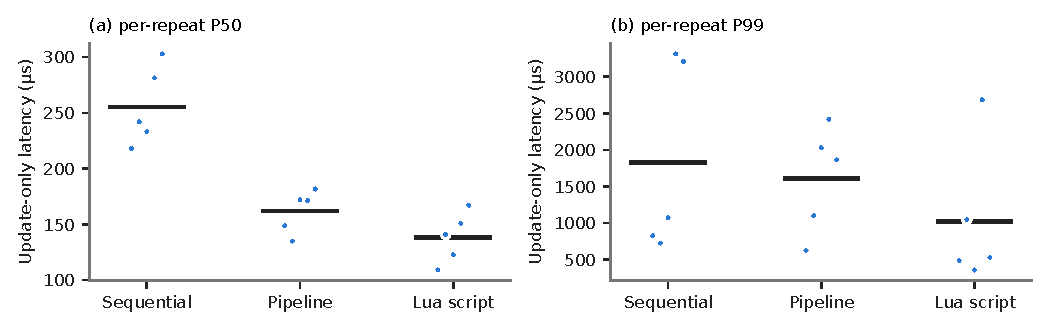
\includegraphics[width=0.9\linewidth]{figS_update_cost.pdf}
\caption{Update-only latency per repeat in \emph{microseconds}; bars mark means over five repeats. Not end-to-end inference latency.}\label{fig:update}
\end{figure}

\begin{table}[h]
\centering\small
\caption{Per-repeat update-only quantiles in \emph{microseconds} (HF7 interpolation).}\label{tab:update_rep}
\begin{tabular}{lrrr}
\toprule
Method & Repeat & P50 ($\mu$s) & P99 ($\mu$s) \\
\midrule
lua & 0 & 109.1 & 484.8 \\
lua & 1 & 141.0 & 1045.4 \\
lua & 2 & 122.8 & 356.1 \\
lua & 3 & 150.9 & 2685.2 \\
lua & 4 & 167.1 & 526.4 \\
pipeline & 0 & 148.8 & 622.7 \\
pipeline & 1 & 134.9 & 1099.4 \\
pipeline & 2 & 172.0 & 2028.6 \\
pipeline & 3 & 171.4 & 2419.0 \\
pipeline & 4 & 181.7 & 1862.5 \\
sequential & 0 & 218.2 & 824.5 \\
sequential & 1 & 242.0 & 723.0 \\
sequential & 2 & 233.2 & 1070.6 \\
sequential & 3 & 281.3 & 3312.7 \\
sequential & 4 & 302.8 & 3209.5 \\
\bottomrule
\end{tabular}
\end{table}

%% ------------------------------------------------------------------
\section{Repeat-level latency values}
\label{sec:repeats}
\paragraph{Controlled replication.} Table~\ref{tab:orig_rep} lists the per-repeat P50 and P99 of each path and the paired ratio for the two-environment replication (XGBoost, $W=30$; 5,000 measured requests per path and repeat; 300,000 records in total; no failures). Repeat indices are those of the run records.

\begin{table}[h]
\centering\small
\caption{Controlled replication, per repeat. Ratio = P99(B1)/P99(A).}\label{tab:orig_rep}
\begin{tabular}{lrrrrrrrrr}
\toprule
 & & & \multicolumn{3}{c}{P50 (ms)} & \multicolumn{3}{c}{P99 (ms)} & \\
\cmidrule(lr){4-6}\cmidrule(lr){7-9}
Env. & $K$ & Rep. & A & B1 & B2 & A & B1 & B2 & Ratio \\
\midrule
Cloud & 1 & 0 & 0.860 & 1.127 & 0.636 & 1.930 & 3.019 & 1.368 & 1.564 \\
Cloud & 1 & 1 & 0.843 & 1.058 & 0.662 & 1.952 & 2.407 & 1.395 & 1.233 \\
Cloud & 1 & 2 & 0.860 & 1.091 & 0.599 & 1.740 & 2.605 & 1.364 & 1.497 \\
Cloud & 1 & 3 & 0.820 & 1.072 & 0.605 & 1.686 & 2.158 & 1.346 & 1.280 \\
Cloud & 1 & 4 & 0.770 & 1.021 & 0.596 & 1.608 & 1.920 & 1.349 & 1.194 \\
Cloud & 100 & 0 & 0.841 & 1.088 & 0.606 & 1.819 & 2.256 & 1.309 & 1.241 \\
Cloud & 100 & 1 & 0.845 & 1.038 & 0.625 & 1.724 & 2.014 & 1.456 & 1.168 \\
Cloud & 100 & 2 & 0.840 & 1.074 & 0.621 & 1.716 & 2.147 & 1.581 & 1.251 \\
Cloud & 100 & 3 & 0.904 & 1.110 & 0.631 & 2.014 & 2.309 & 1.502 & 1.146 \\
Cloud & 100 & 4 & 0.880 & 1.032 & 0.661 & 2.168 & 2.060 & 1.551 & 0.950 \\
Laptop & 1 & 0 & 1.164 & 1.258 & 0.664 & 6.863 & 4.989 & 2.396 & 0.727 \\
Laptop & 1 & 1 & 0.946 & 1.267 & 0.566 & 2.856 & 7.889 & 2.547 & 2.763 \\
Laptop & 1 & 2 & 0.901 & 1.131 & 0.595 & 3.724 & 3.308 & 2.072 & 0.888 \\
Laptop & 1 & 3 & 0.943 & 1.185 & 0.608 & 4.528 & 3.372 & 2.449 & 0.745 \\
Laptop & 1 & 4 & 0.921 & 1.166 & 0.573 & 2.400 & 3.034 & 2.149 & 1.264 \\
Laptop & 100 & 0 & 0.922 & 1.205 & 0.716 & 2.969 & 4.260 & 2.395 & 1.435 \\
Laptop & 100 & 1 & 0.965 & 1.135 & 0.579 & 2.639 & 6.085 & 2.037 & 2.306 \\
Laptop & 100 & 2 & 0.869 & 1.274 & 0.593 & 3.599 & 3.285 & 3.074 & 0.913 \\
Laptop & 100 & 3 & 0.877 & 1.254 & 0.579 & 2.748 & 3.683 & 3.357 & 1.340 \\
Laptop & 100 & 4 & 0.855 & 1.244 & 0.551 & 2.070 & 4.059 & 2.046 & 1.961 \\
\bottomrule
\end{tabular}
\end{table}

\paragraph{Client CPU restriction (pre-specified).} Cloud environment, $K=1$, $W=30$, XGBoost, client affinity restricted to one or two cores with Redis unrestricted; 150,000 records, no failures; Stage-2 rate 37.4\%. Prediction: the median ratio stays above one in both conditions (met).

\begin{table}[h]
\centering\small
\caption{Client CPU restriction, per repeat: P99 (ms) and ratio P99(B1)/P99(A). Medians: 1.27 (one core), 1.19 (two cores); B2 CV 0.11 and 0.08.}\label{tab:rc}
\begin{tabular}{lrrrrr}
\toprule
Client cores & Repeat & A & B1 & B2 & Ratio \\
\midrule
1 & 0 & 1.869 & 2.434 & 1.216 & 1.302 \\
1 & 1 & 1.582 & 2.010 & 1.521 & 1.270 \\
1 & 2 & 2.137 & 1.954 & 1.401 & 0.915 \\
1 & 3 & 1.690 & 2.145 & 1.278 & 1.269 \\
1 & 4 & 2.171 & 2.539 & 1.577 & 1.170 \\
2 & 0 & 1.593 & 2.278 & 1.536 & 1.431 \\
2 & 1 & 2.058 & 1.814 & 1.269 & 0.881 \\
2 & 2 & 1.510 & 2.368 & 1.383 & 1.569 \\
2 & 3 & 1.871 & 1.869 & 1.324 & 0.999 \\
2 & 4 & 1.934 & 2.305 & 1.293 & 1.192 \\
\bottomrule
\end{tabular}
\end{table}

\paragraph{Breadth, cloud container of the replication type with the original input.} Run directory \path{extension_20261012T185318Z_07aeb598} (env label \path{cloudcontainer_original75}); status \texttt{complete}; 450,000 measured requests, no failures; B1 and B2 agreed with A on the predicted label and on the Stage-2 decision at all 150,000 request positions. Host: a new cloud container of the same type as the replication's cloud environment (Intel Xeon 2.10\,GHz, 2 vCPU, about 8\,GB, Firecracker-based VM, Linux 6.18.44), not the same instance; Python 3.13.16, NumPy 2.5.3, pandas 3.0.5, scikit-learn 1.6.1, XGBoost 3.4.1, PyTorch 2.14.1; Redis server 7.0.15 (Ubuntu package) started for the run on a dedicated port with RDB saving and the append-only file disabled, direct loopback. Hash check: \texttt{all\_match}. The input files were supplied by the authors for this run. Mean host utilisation was 42--48\% per cell (one of two vCPUs corresponds to 50\%). The run was executed by the revision assistant in its sandbox on 2026-10-12 (18:53--19:03 UTC), with no other measurement running. Tables~\ref{tab:cloud_p50} and~\ref{tab:cloud_rep} give the P50 summary and per-repeat values.

\begin{table}[h]
\centering\small
\caption{Breadth, cloud container: mean over five repeats of the per-repeat P50 (ms) and ratio of the means. Descriptive; not a pre-specified rule.}\label{tab:cloud_p50}
\begin{tabular}{lrrrrr}
\toprule
Model & $K$ & A & B1 & B2 & B1/A \\
\midrule
Logistic & 1 & 0.340 & 0.592 & 0.158 & 1.74 \\
Logistic & 100 & 0.322 & 0.549 & 0.157 & 1.70 \\
Random forest & 1 & 1.159 & 1.371 & 0.917 & 1.18 \\
Random forest & 100 & 1.302 & 1.575 & 0.968 & 1.21 \\
XGBoost & 1 & 0.888 & 1.142 & 0.611 & 1.29 \\
XGBoost & 100 & 0.875 & 1.132 & 0.648 & 1.29 \\
\bottomrule
\end{tabular}
\end{table}

\begin{longtable}{lrrrrrrrrr}
\caption{Breadth, cloud container, per repeat. Ratio = P99(B1)/P99(A).}\label{tab:cloud_rep}\\
\toprule
 & & & \multicolumn{3}{c}{P50 (ms)} & \multicolumn{3}{c}{P99 (ms)} & \\
\cmidrule(lr){4-6}\cmidrule(lr){7-9}
Model & $K$ & Rep. & A & B1 & B2 & A & B1 & B2 & Ratio \\
\midrule
\endfirsthead
\toprule
Model & $K$ & Rep. & A & B1 & B2 & A & B1 & B2 & Ratio \\
\midrule
\endhead
Logistic & 1 & 0 & 0.346 & 0.557 & 0.156 & 0.858 & 1.518 & 0.443 & 1.769 \\
Logistic & 1 & 1 & 0.345 & 0.605 & 0.154 & 0.896 & 1.471 & 0.399 & 1.641 \\
Logistic & 1 & 2 & 0.305 & 0.604 & 0.142 & 0.715 & 1.464 & 0.363 & 2.049 \\
Logistic & 1 & 3 & 0.342 & 0.544 & 0.148 & 0.826 & 1.334 & 0.382 & 1.615 \\
Logistic & 1 & 4 & 0.364 & 0.647 & 0.190 & 1.099 & 1.875 & 0.771 & 1.706 \\
Logistic & 100 & 0 & 0.296 & 0.550 & 0.151 & 0.679 & 1.183 & 0.469 & 1.741 \\
Logistic & 100 & 1 & 0.341 & 0.574 & 0.150 & 0.969 & 1.361 & 0.451 & 1.404 \\
Logistic & 100 & 2 & 0.303 & 0.525 & 0.160 & 0.732 & 1.185 & 0.462 & 1.618 \\
Logistic & 100 & 3 & 0.310 & 0.533 & 0.153 & 0.864 & 1.152 & 0.384 & 1.334 \\
Logistic & 100 & 4 & 0.360 & 0.565 & 0.168 & 1.024 & 1.521 & 0.453 & 1.486 \\
Random forest & 1 & 0 & 1.122 & 1.411 & 1.128 & 3.068 & 3.197 & 2.806 & 1.042 \\
Random forest & 1 & 1 & 1.393 & 1.485 & 0.857 & 3.662 & 3.256 & 2.318 & 0.889 \\
Random forest & 1 & 2 & 1.116 & 1.339 & 0.869 & 3.027 & 3.245 & 2.701 & 1.072 \\
Random forest & 1 & 3 & 1.059 & 1.268 & 0.902 & 3.077 & 3.087 & 2.453 & 1.003 \\
Random forest & 1 & 4 & 1.103 & 1.353 & 0.827 & 2.959 & 3.425 & 2.371 & 1.157 \\
Random forest & 100 & 0 & 1.382 & 1.450 & 0.952 & 3.336 & 3.105 & 2.533 & 0.931 \\
Random forest & 100 & 1 & 1.345 & 1.540 & 1.046 & 3.738 & 3.519 & 2.918 & 0.942 \\
Random forest & 100 & 2 & 1.159 & 1.674 & 0.998 & 3.089 & 3.356 & 2.590 & 1.086 \\
Random forest & 100 & 3 & 1.256 & 1.653 & 0.983 & 2.874 & 3.251 & 2.554 & 1.131 \\
Random forest & 100 & 4 & 1.368 & 1.556 & 0.862 & 3.845 & 3.486 & 2.250 & 0.907 \\
XGBoost & 1 & 0 & 0.919 & 1.176 & 0.597 & 1.983 & 2.372 & 1.444 & 1.197 \\
XGBoost & 1 & 1 & 0.884 & 1.171 & 0.599 & 1.913 & 2.421 & 1.437 & 1.265 \\
XGBoost & 1 & 2 & 0.919 & 1.117 & 0.660 & 2.075 & 2.134 & 1.637 & 1.028 \\
XGBoost & 1 & 3 & 0.859 & 1.090 & 0.602 & 1.948 & 2.114 & 1.501 & 1.085 \\
XGBoost & 1 & 4 & 0.861 & 1.155 & 0.597 & 1.886 & 2.537 & 1.408 & 1.345 \\
XGBoost & 100 & 0 & 0.937 & 1.120 & 0.623 & 2.203 & 2.203 & 1.387 & 1.000 \\
XGBoost & 100 & 1 & 0.841 & 1.135 & 0.651 & 1.813 & 2.251 & 1.500 & 1.242 \\
XGBoost & 100 & 2 & 0.871 & 1.122 & 0.670 & 2.053 & 2.247 & 1.653 & 1.094 \\
XGBoost & 100 & 3 & 0.870 & 1.151 & 0.650 & 1.940 & 2.356 & 1.732 & 1.214 \\
XGBoost & 100 & 4 & 0.857 & 1.132 & 0.646 & 1.867 & 2.455 & 1.710 & 1.315 \\
\bottomrule
\end{longtable}

\paragraph{Breadth, replication laptop with the original input, first occasion.} Run directory \path{extension_20261011T183015Z_1fa8e163}, env label \path{seonwoo_wsl_original75}; status \texttt{complete}; 450,000 measured requests, no failures; B1 and B2 agreed with A on the predicted label and on the Stage-2 decision at all 150,000 request positions. Host: the replication laptop (Intel Core 5 210H, 12 logical CPUs, WSL2, Linux 6.18.35.2), Python 3.13.16, NumPy 2.5.3, scikit-learn 1.6.1, XGBoost 3.4.1, redis-py 8.1.0, PyTorch 2.14.1 (CPU), Redis server 8.0.5 started for the run on a dedicated port with RDB saving and the append-only file disabled, direct loopback. Preflight and the original driver's hash check reported \texttt{all\_match} for code, artefacts, the 75 input files and the input array. The driver's background CPU sampler recorded a mean host utilisation of 7.8--8.8\% per cell (one of 12 logical CPUs corresponds to 8.3\%). The run was started from the authors' breadth script on 2026-10-11 (18:30--18:42 UTC). Tables~\ref{tab:lap_p50} and~\ref{tab:lap_rep} give the P50 summary and per-repeat values.

\begin{table}[h]
\centering\small
\caption{Breadth, laptop, first occasion: mean over five repeats of the per-repeat P50 (ms) and ratio of the means. Descriptive; not a pre-specified rule.}\label{tab:lap_p50}
\begin{tabular}{lrrrrr}
\toprule
Model & $K$ & A & B1 & B2 & B1/A \\
\midrule
Logistic & 1 & 0.395 & 0.635 & 0.129 & 1.61 \\
Logistic & 100 & 0.385 & 0.727 & 0.148 & 1.89 \\
Random forest & 1 & 1.379 & 1.634 & 0.819 & 1.18 \\
Random forest & 100 & 1.405 & 1.716 & 1.018 & 1.22 \\
XGBoost & 1 & 0.900 & 1.195 & 0.525 & 1.33 \\
XGBoost & 100 & 0.905 & 1.339 & 0.567 & 1.48 \\
\bottomrule
\end{tabular}
\end{table}

\begin{longtable}{lrrrrrrrrr}
\caption{Breadth, laptop, first occasion, per repeat. Ratio = P99(B1)/P99(A).}\label{tab:lap_rep}\\
\toprule
 & & & \multicolumn{3}{c}{P50 (ms)} & \multicolumn{3}{c}{P99 (ms)} & \\
\cmidrule(lr){4-6}\cmidrule(lr){7-9}
Model & $K$ & Rep. & A & B1 & B2 & A & B1 & B2 & Ratio \\
\midrule
\endfirsthead
\toprule
Model & $K$ & Rep. & A & B1 & B2 & A & B1 & B2 & Ratio \\
\midrule
\endhead
Logistic & 1 & 0 & 0.379 & 0.612 & 0.122 & 0.812 & 2.731 & 0.475 & 3.365 \\
Logistic & 1 & 1 & 0.378 & 0.587 & 0.154 & 1.806 & 1.654 & 0.631 & 0.916 \\
Logistic & 1 & 2 & 0.429 & 0.683 & 0.116 & 1.453 & 2.858 & 0.595 & 1.967 \\
Logistic & 1 & 3 & 0.437 & 0.613 & 0.125 & 2.641 & 2.057 & 0.985 & 0.779 \\
Logistic & 1 & 4 & 0.350 & 0.680 & 0.129 & 1.341 & 3.238 & 0.635 & 2.415 \\
Logistic & 100 & 0 & 0.340 & 0.700 & 0.132 & 0.831 & 3.837 & 0.418 & 4.619 \\
Logistic & 100 & 1 & 0.412 & 0.798 & 0.142 & 1.554 & 5.077 & 1.036 & 3.268 \\
Logistic & 100 & 2 & 0.363 & 0.588 & 0.173 & 1.391 & 1.260 & 0.633 & 0.905 \\
Logistic & 100 & 3 & 0.356 & 0.571 & 0.144 & 0.883 & 1.761 & 0.626 & 1.995 \\
Logistic & 100 & 4 & 0.453 & 0.979 & 0.146 & 2.827 & 5.138 & 0.623 & 1.818 \\
Random forest & 1 & 0 & 1.521 & 1.958 & 0.850 & 8.351 & 8.436 & 4.579 & 1.010 \\
Random forest & 1 & 1 & 1.346 & 1.432 & 0.695 & 7.338 & 5.164 & 3.092 & 0.704 \\
Random forest & 1 & 2 & 1.613 & 1.628 & 1.015 & 6.831 & 6.116 & 4.449 & 0.895 \\
Random forest & 1 & 3 & 1.126 & 1.497 & 0.764 & 3.589 & 3.925 & 2.799 & 1.094 \\
Random forest & 1 & 4 & 1.291 & 1.653 & 0.772 & 6.514 & 7.567 & 3.887 & 1.162 \\
Random forest & 100 & 0 & 1.606 & 1.797 & 1.065 & 6.785 & 6.325 & 5.903 & 0.932 \\
Random forest & 100 & 1 & 1.621 & 1.859 & 0.911 & 9.354 & 12.712 & 2.668 & 1.359 \\
Random forest & 100 & 2 & 1.360 & 1.606 & 1.051 & 5.179 & 4.739 & 5.161 & 0.915 \\
Random forest & 100 & 3 & 1.348 & 1.571 & 1.051 & 4.123 & 3.829 & 3.396 & 0.929 \\
Random forest & 100 & 4 & 1.093 & 1.749 & 1.010 & 2.473 & 9.669 & 3.809 & 3.910 \\
XGBoost & 1 & 0 & 0.900 & 1.217 & 0.578 & 4.398 & 4.942 & 4.034 & 1.124 \\
XGBoost & 1 & 1 & 0.935 & 1.166 & 0.519 & 3.968 & 3.584 & 3.018 & 0.903 \\
XGBoost & 1 & 2 & 0.937 & 1.366 & 0.487 & 3.830 & 5.901 & 3.016 & 1.541 \\
XGBoost & 1 & 3 & 0.844 & 1.090 & 0.500 & 2.431 & 5.098 & 1.289 & 2.097 \\
XGBoost & 1 & 4 & 0.884 & 1.136 & 0.539 & 4.528 & 4.779 & 2.231 & 1.055 \\
XGBoost & 100 & 0 & 0.973 & 1.167 & 0.519 & 4.041 & 3.463 & 2.022 & 0.857 \\
XGBoost & 100 & 1 & 0.823 & 1.764 & 0.556 & 2.498 & 7.894 & 2.397 & 3.160 \\
XGBoost & 100 & 2 & 0.833 & 1.504 & 0.630 & 1.867 & 7.760 & 1.833 & 4.157 \\
XGBoost & 100 & 3 & 1.004 & 1.060 & 0.584 & 6.620 & 3.532 & 4.294 & 0.534 \\
XGBoost & 100 & 4 & 0.892 & 1.200 & 0.543 & 3.305 & 3.876 & 1.675 & 1.173 \\
\bottomrule
\end{longtable}

\paragraph{Breadth, replication laptop with the original input, second occasion.} Run directory \path{extension_20261012T190558Z_afd135a9}, env label \path{seonwoo_wsl_original75}; same command, host, software versions and Redis 8.0.5 as the first occasion; run on 2026-10-12 (19:06--19:19 UTC); status \texttt{complete}; \texttt{all\_match}; 450,000 measured requests, no failures, no label or Stage-2 mismatches. The driver's background CPU sampler recorded a mean host utilisation of 7.1--8.1\% per cell. Table~\ref{tab:lap2_rep} gives the per-repeat values, recomputed from the raw records.

\begin{longtable}{lrrrrrrrrr}
\caption{Breadth, laptop, second occasion, per repeat. Ratio = P99(B1)/P99(A).}\label{tab:lap2_rep}\\
\toprule
 & & & \multicolumn{3}{c}{P50 (ms)} & \multicolumn{3}{c}{P99 (ms)} & \\
\cmidrule(lr){4-6}\cmidrule(lr){7-9}
Model & $K$ & Rep. & A & B1 & B2 & A & B1 & B2 & Ratio \\
\midrule
\endfirsthead
\toprule
Model & $K$ & Rep. & A & B1 & B2 & A & B1 & B2 & Ratio \\
\midrule
\endhead
Logistic & 1 & 0 & 0.485 & 0.810 & 0.161 & 1.265 & 2.380 & 0.593 & 1.881 \\
Logistic & 1 & 1 & 0.561 & 1.063 & 0.179 & 1.555 & 4.756 & 1.035 & 3.058 \\
Logistic & 1 & 2 & 0.455 & 0.894 & 0.148 & 1.122 & 3.323 & 0.658 & 2.963 \\
Logistic & 1 & 3 & 0.605 & 0.883 & 0.170 & 1.767 & 2.301 & 0.623 & 1.303 \\
Logistic & 1 & 4 & 0.610 & 1.018 & 0.146 & 1.864 & 4.005 & 0.563 & 2.149 \\
Logistic & 100 & 0 & 0.570 & 0.851 & 0.205 & 1.277 & 1.913 & 0.871 & 1.499 \\
Logistic & 100 & 1 & 0.573 & 0.938 & 0.189 & 1.451 & 4.266 & 0.705 & 2.940 \\
Logistic & 100 & 2 & 0.542 & 0.860 & 0.195 & 1.310 & 3.194 & 0.761 & 2.439 \\
Logistic & 100 & 3 & 0.632 & 0.962 & 0.191 & 2.389 & 3.227 & 0.713 & 1.351 \\
Logistic & 100 & 4 & 0.538 & 0.933 & 0.200 & 1.399 & 2.090 & 0.919 & 1.493 \\
Random forest & 1 & 0 & 1.354 & 1.793 & 0.888 & 3.469 & 4.465 & 2.664 & 1.287 \\
Random forest & 1 & 1 & 1.625 & 1.774 & 0.879 & 6.625 & 4.372 & 2.716 & 0.660 \\
Random forest & 1 & 2 & 1.759 & 1.967 & 0.975 & 7.263 & 8.098 & 3.274 & 1.115 \\
Random forest & 1 & 3 & 1.458 & 1.953 & 1.116 & 3.502 & 4.038 & 3.240 & 1.153 \\
Random forest & 1 & 4 & 1.679 & 2.199 & 1.180 & 5.556 & 7.572 & 4.178 & 1.363 \\
Random forest & 100 & 0 & 1.785 & 2.156 & 1.345 & 4.624 & 7.055 & 5.212 & 1.526 \\
Random forest & 100 & 1 & 1.666 & 2.190 & 1.367 & 3.875 & 8.217 & 7.278 & 2.121 \\
Random forest & 100 & 2 & 1.870 & 1.981 & 1.339 & 7.169 & 5.356 & 4.257 & 0.747 \\
Random forest & 100 & 3 & 1.731 & 2.121 & 1.347 & 5.917 & 4.819 & 4.481 & 0.814 \\
Random forest & 100 & 4 & 1.291 & 1.626 & 0.990 & 2.841 & 3.558 & 2.646 & 1.252 \\
XGBoost & 1 & 0 & 1.002 & 1.329 & 0.594 & 2.348 & 5.216 & 1.727 & 2.222 \\
XGBoost & 1 & 1 & 1.189 & 1.447 & 0.650 & 4.484 & 5.487 & 2.612 & 1.224 \\
XGBoost & 1 & 2 & 1.117 & 1.479 & 0.609 & 3.563 & 3.742 & 2.023 & 1.050 \\
XGBoost & 1 & 3 & 1.184 & 1.776 & 0.699 & 2.506 & 4.100 & 2.070 & 1.636 \\
XGBoost & 1 & 4 & 1.033 & 1.475 & 0.608 & 2.341 & 3.569 & 1.591 & 1.524 \\
XGBoost & 100 & 0 & 1.273 & 1.758 & 0.847 & 3.033 & 4.458 & 2.508 & 1.470 \\
XGBoost & 100 & 1 & 1.305 & 1.540 & 0.689 & 5.781 & 6.336 & 1.978 & 1.096 \\
XGBoost & 100 & 2 & 1.287 & 1.727 & 0.734 & 5.808 & 8.746 & 2.771 & 1.506 \\
XGBoost & 100 & 3 & 1.233 & 1.427 & 0.743 & 6.379 & 3.173 & 2.234 & 0.497 \\
XGBoost & 100 & 4 & 0.988 & 1.306 & 0.622 & 2.163 & 2.723 & 1.681 & 1.259 \\
\bottomrule
\end{longtable}

\paragraph{Breadth, shared host with the November 2025 input.} Run directory \path{extension_20261011T115213Z_9ba1751a}; status \texttt{complete}; 30 cells (3 models $\times$ $K\in\{1,100\}$ $\times$ 5 repeats), 450,000 measured requests, no failures; B1 and B2 agreed with A on the predicted label and on the Stage-2 decision at all 150,000 request positions. Environment: AMD EPYC 9V74, cgroup quota of 8 CPUs and 8\,GiB memory (9 logical CPUs visible), Linux 6.18, Python 3.12.14, NumPy 2.3.5, scikit-learn 1.6.1, XGBoost 3.4.1, redis-py 8.1.0; Redis server 6.2.14 (the executable distributed with the \texttt{redislite} package, contacted directly over TCP loopback, Lua executed by the server; not a simulator), append-only file disabled (\texttt{aof\_enabled=0} in the metadata); RDB snapshotting is not configured by the driver and its configuration was not recorded. Model loading read the stored thresholds and both stages reported one thread. Model order was permuted per $K$ and repeat with a recorded seed; path order used the original seed rule. The host was shared with documentation work during the run, with short plotting and host-inspection activity near the last conditions; all observations were kept and no condition was re-run. Input: Binance BTCUSDT one-second features, 2,438 files, 2,437,999 rows, 2025-11-01 00:00:00 to 2025-11-30 23:59:59 UTC, timestamps non-decreasing with 168 duplicate timestamps in the full archive and none in the first 8,300 rows; no row was dropped or re-sorted. $K=1$ used the first 5,230 rows and $K=100$ the first 8,200 rows ($L=30+\lceil5200/100\rceil=82$). None of the 2,438 file hashes matches the 75 files of the controlled replication. Tables~\ref{tab:ext_p50} and~\ref{tab:ext_rep} give the P50 summary and per-repeat values; Figure~3 of the main paper shows the ratios.

\begin{table}[h]
\centering\small
\caption{Breadth, shared host: mean over five repeats of the per-repeat P50 (ms) and ratio of the means. Descriptive; not a pre-specified rule.}\label{tab:ext_p50}
\begin{tabular}{lrrrrr}
\toprule
Model & $K$ & A & B1 & B2 & B1/A \\
\midrule
Logistic & 1 & 0.291 & 0.456 & 0.155 & 1.57 \\
Logistic & 100 & 0.288 & 0.445 & 0.146 & 1.54 \\
Random forest & 1 & 1.035 & 1.220 & 0.894 & 1.18 \\
Random forest & 100 & 0.992 & 1.179 & 0.856 & 1.19 \\
XGBoost & 1 & 0.519 & 0.695 & 0.400 & 1.34 \\
XGBoost & 100 & 0.515 & 0.657 & 0.401 & 1.28 \\
\bottomrule
\end{tabular}
\end{table}

\begin{longtable}{lrrrrrrrrr}
\caption{Breadth, shared host, per repeat. Ratio = P99(B1)/P99(A).}\label{tab:ext_rep}\\
\toprule
 & & & \multicolumn{3}{c}{P50 (ms)} & \multicolumn{3}{c}{P99 (ms)} & \\
\cmidrule(lr){4-6}\cmidrule(lr){7-9}
Model & $K$ & Rep. & A & B1 & B2 & A & B1 & B2 & Ratio \\
\midrule
\endfirsthead
\toprule
Model & $K$ & Rep. & A & B1 & B2 & A & B1 & B2 & Ratio \\
\midrule
\endhead
Logistic & 1 & 0 & 0.281 & 0.479 & 0.145 & 0.609 & 0.784 & 0.393 & 1.289 \\
Logistic & 1 & 1 & 0.276 & 0.384 & 0.142 & 0.527 & 0.715 & 0.338 & 1.358 \\
Logistic & 1 & 2 & 0.321 & 0.506 & 0.200 & 0.771 & 0.937 & 0.526 & 1.215 \\
Logistic & 1 & 3 & 0.259 & 0.497 & 0.149 & 0.616 & 0.957 & 0.457 & 1.555 \\
Logistic & 1 & 4 & 0.316 & 0.413 & 0.140 & 0.540 & 0.749 & 0.294 & 1.388 \\
Logistic & 100 & 0 & 0.300 & 0.412 & 0.146 & 0.550 & 0.724 & 0.400 & 1.317 \\
Logistic & 100 & 1 & 0.277 & 0.407 & 0.144 & 0.620 & 0.761 & 0.447 & 1.228 \\
Logistic & 100 & 2 & 0.311 & 0.495 & 0.143 & 0.634 & 0.849 & 0.390 & 1.339 \\
Logistic & 100 & 3 & 0.316 & 0.496 & 0.154 & 0.684 & 0.849 & 0.590 & 1.241 \\
Logistic & 100 & 4 & 0.238 & 0.416 & 0.143 & 0.510 & 0.868 & 0.353 & 1.701 \\
Random forest & 1 & 0 & 1.052 & 1.114 & 0.847 & 1.473 & 2.351 & 1.405 & 1.596 \\
Random forest & 1 & 1 & 0.974 & 1.233 & 0.854 & 2.125 & 1.813 & 1.324 & 0.853 \\
Random forest & 1 & 2 & 0.993 & 1.224 & 0.873 & 1.574 & 3.192 & 1.748 & 2.028 \\
Random forest & 1 & 3 & 1.118 & 1.255 & 0.957 & 3.671 & 2.521 & 3.032 & 0.687 \\
Random forest & 1 & 4 & 1.036 & 1.273 & 0.938 & 1.418 & 2.597 & 2.963 & 1.831 \\
Random forest & 100 & 0 & 0.975 & 1.236 & 0.850 & 1.757 & 1.921 & 1.584 & 1.093 \\
Random forest & 100 & 1 & 0.993 & 1.131 & 0.863 & 1.632 & 2.079 & 1.488 & 1.274 \\
Random forest & 100 & 2 & 1.061 & 1.127 & 0.839 & 2.143 & 1.677 & 1.344 & 0.782 \\
Random forest & 100 & 3 & 0.964 & 1.207 & 0.862 & 1.388 & 1.951 & 2.106 & 1.406 \\
Random forest & 100 & 4 & 0.968 & 1.193 & 0.869 & 1.766 & 2.600 & 1.760 & 1.472 \\
XGBoost & 1 & 0 & 0.534 & 0.666 & 0.402 & 1.098 & 1.174 & 0.805 & 1.069 \\
XGBoost & 1 & 1 & 0.507 & 0.746 & 0.395 & 0.913 & 1.037 & 0.748 & 1.135 \\
XGBoost & 1 & 2 & 0.520 & 0.663 & 0.399 & 0.831 & 1.593 & 0.842 & 1.917 \\
XGBoost & 1 & 3 & 0.519 & 0.744 & 0.403 & 2.149 & 1.729 & 0.824 & 0.804 \\
XGBoost & 1 & 4 & 0.515 & 0.656 & 0.400 & 0.899 & 1.116 & 0.859 & 1.242 \\
XGBoost & 100 & 0 & 0.519 & 0.693 & 0.395 & 0.896 & 1.322 & 0.716 & 1.476 \\
XGBoost & 100 & 1 & 0.494 & 0.625 & 0.398 & 0.849 & 0.991 & 0.810 & 1.167 \\
XGBoost & 100 & 2 & 0.530 & 0.649 & 0.396 & 0.910 & 1.013 & 0.949 & 1.114 \\
XGBoost & 100 & 3 & 0.547 & 0.632 & 0.419 & 0.860 & 1.181 & 1.218 & 1.373 \\
XGBoost & 100 & 4 & 0.484 & 0.688 & 0.396 & 0.790 & 1.083 & 0.746 & 1.371 \\
\bottomrule
\end{longtable}

%% ------------------------------------------------------------------
\section{Window sweep and memory details}
\label{sec:window}
Per-repeat P99(B1)/P99(A) ratios of the window sweep (cloud, $K=1$, XGBoost, client restricted to two cores; repeats 0--4) are given in Table~\ref{tab:win_rep}. All 20 exceed one; the medians are 1.30, 1.30, 1.14 and 1.47 (Spearman $\rho=0.40$ against $W$; the pre-specified descriptive prediction of an increasing tail ratio is met in sign only). When $W$ changes, the fill length and the scheduled row offsets change too, so differences in total latency across $W$ are not a pure effect of $W$. The memory experiment used one key per $W$, written through the Lua writer without inference; \texttt{MEMORY USAGE ... SAMPLES 0} was identical in all five repeats at every checkpoint (100 checkpoints). The logical payload is $4d\min(N,W)$ bytes; the measured value additionally includes per-entry, object and key-name overhead and depends on the Redis build, encoding and allocator.

\begin{table}[h]
\centering\small
\caption{Window sweep: per-repeat P99(B1)/P99(A).}\label{tab:win_rep}
\begin{tabular}{rrrrrr}
\toprule
$W$ & Rep.~0 & Rep.~1 & Rep.~2 & Rep.~3 & Rep.~4 \\
\midrule
10 & 1.295 & 1.335 & 1.407 & 1.185 & 1.090 \\
30 & 1.159 & 1.083 & 1.512 & 1.427 & 1.300 \\
60 & 1.523 & 1.108 & 1.512 & 1.144 & 1.138 \\
120 & 1.657 & 1.573 & 1.475 & 1.346 & 1.026 \\
\bottomrule
\end{tabular}
\end{table}

%% ------------------------------------------------------------------
\section{Earlier evaluation: historical summaries (not evidence)}
\label{sec:breadth}
\paragraph{Provenance status: historical, unmatched.} The tables below are the aggregates reported in the previous version of the manuscript for the earlier implementation (non-atomic pipelined update, Redis in Docker on macOS, Python 3.11.13, NumPy 1.26.4, scikit-learn 1.6.1, XGBoost 3.1.2, library-default threading). They are reproduced verbatim for transparency. They were \emph{not} independently recomputed, and they are not used to support any claim in the main paper, for the following reasons established in the provenance audit:
\begin{itemize}
\item The latency files that exist in the repository (\path{results/latency_k_<model>.csv} and \path{latency_k_<model>_2025_11.csv} for the three models, 30,000 rows each; \texttt{latency\_k\_sweep\_FULL.csv}, 90,000 rows; \texttt{latency\_multisymbol\_mixed.csv}, 24,000 rows) all record a single gate threshold of 0.6731, whereas the tables below were reported at the model-specific thresholds of Table~\ref{tab:thr}.
\item In those files, the \texttt{trial} column is a request index with 2,000 values, not an outer repetition; the reported protocol was five trials of 500 warm-up and 5,000 measured ticks, and the benchmark defaults are 200 and 2,000.
\item The repository documentation states that these files predate later fixes to the benchmark code.
\item Scripts recovered from an older branch (\texttt{bench\_2025\_05.py}, \texttt{bench\_nov2025.py}) implement five outer trials but belong to differently named experiments and record only P99 per trial and $K$; they cannot be matched to the tables below, and git timestamps cannot establish the dates of the reported runs.
\item No original plotting script, code version or artefact hash for these runs was found.
\end{itemize}
The reported data periods (BTCUSDT 1--2 and 1--14 August 2026, ten assets on 1--2 August 2026, and 1--7 September 2026) are as stated by the authors and were not verified. ``Reduction'' is $1-L_A/L_{B1}$; ``TPS gain'' is the throughput ratio A/B1.

\begin{table}[h]\centering\small
\caption{HISTORICAL, NOT RECOMPUTED. Earlier operating-point comparison at the stored thresholds: mean and P99 of A/B1 in ms (slash, not a ratio) with A's reduction.}
\begin{tabular*}{\linewidth}{@{\extracolsep{\fill}}l r r l l r@{}}
\toprule
Model & $K$ & Stage-2 (\%) & Mean A/B1 (reduction) & P99 A/B1 (reduction) & TPS gain \\
\midrule
Logistic & 1 & 62.5 & 1.005/1.740 (42.2\%) & 2.245/4.240 (47.0\%) & 1.71$\times$ \\
Logistic & 5 & 91.5 & 0.945/1.616 (41.5\%) & 1.476/2.654 (44.4\%) & 1.70$\times$ \\
Logistic & 10 & 88.2 & 0.920/1.552 (40.7\%) & 1.431/2.395 (40.3\%) & 1.68$\times$ \\
Logistic & 20 & 90.5 & 0.920/1.554 (40.8\%) & 1.499/2.326 (35.5\%) & 1.68$\times$ \\
Logistic & 50 & 74.8 & 0.912/1.534 (40.5\%) & 1.423/2.495 (43.0\%) & 1.68$\times$ \\
XGBoost & 1 & 56.4 & 1.431/2.235 (36.0\%) & 2.813/3.556 (20.9\%) & 1.56$\times$ \\
XGBoost & 5 & 65.7 & 1.630/2.404 (32.2\%) & 3.558/4.712 (24.5\%) & 1.45$\times$ \\
XGBoost & 10 & 69.2 & 1.657/2.890 (42.7\%) & 3.425/6.910 (50.4\%) & 1.73$\times$ \\
XGBoost & 20 & 68.1 & 1.897/2.573 (26.3\%) & 4.457/4.522 (1.4\%) & 1.37$\times$ \\
XGBoost & 50 & 56.1 & 1.667/2.655 (37.2\%) & 3.280/5.011 (34.5\%) & 1.59$\times$ \\
Random Forest & 1 & 73.2 & 2.413/2.873 (16.0\%) & 4.008/4.419 (9.3\%) & 1.20$\times$ \\
Random Forest & 5 & 86.1 & 2.729/3.183 (14.3\%) & 4.978/5.568 (10.6\%) & 1.17$\times$ \\
Random Forest & 10 & 92.8 & 2.827/3.502 (19.3\%) & 5.605/6.820 (17.8\%) & 1.24$\times$ \\
Random Forest & 20 & 88.9 & 2.646/3.344 (20.9\%) & 5.069/6.832 (25.8\%) & 1.25$\times$ \\
Random Forest & 50 & 72.0 & 2.477/2.988 (17.1\%) & 5.223/5.595 (6.6\%) & 1.21$\times$ \\
\bottomrule
\end{tabular*}
\end{table}

\begin{table}[h]\centering\small
\footnotesize\setlength{\tabcolsep}{3pt}\caption{HISTORICAL, NOT RECOMPUTED. Earlier gating ablation on path A (gate at the stored operating thresholds, labelled ``Cal.'' in the original table, versus always running Stage~2; ``Fixed'' is a high-threshold reference). ``Cal.'' does not imply optimal calibration (Section~\ref{sec:training}).}
\begin{tabular*}{\linewidth}{@{\extracolsep{\fill}}l r r r r r r r@{}}
\toprule
Model & $K$ & Cal. inv. (\%) & Fixed inv. (\%) & Cal. P99 (ms) & Always P99 (ms) & P99 reduction & TPS gain \\
\midrule
Logistic & 1 & 63.3 & 0.02 & 1.581 & 1.817 & 13.0\% & 1.06$\times$ \\
Logistic & 10 & 90.9 & 0.00 & 1.599 & 2.200 & 27.3\% & 1.08$\times$ \\
Logistic & 50 & 90.2 & 0.04 & 1.729 & 1.868 & 7.4\% & 1.03$\times$ \\
XGBoost & 1 & 57.4 & 0.76 & 2.765 & 3.039 & 9.0\% & 1.13$\times$ \\
XGBoost & 10 & 59.4 & 0.64 & 2.384 & 2.817 & 15.4\% & 1.10$\times$ \\
XGBoost & 50 & 59.8 & 0.66 & 2.560 & 2.797 & 8.5\% & 1.09$\times$ \\
Random Forest & 1 & 73.5 & 0.00 & 3.574 & 4.097 & 12.8\% & 1.12$\times$ \\
Random Forest & 10 & 82.2 & 0.00 & 4.107 & 4.150 & 1.0\% & 1.08$\times$ \\
Random Forest & 50 & 80.3 & 0.00 & 4.021 & 5.377 & 25.2\% & 1.16$\times$ \\
\bottomrule
\end{tabular*}
\end{table}

\begin{table}[h]\centering\small
\caption{HISTORICAL, NOT RECOMPUTED. Earlier distinct-asset experiment; $K$ is the number of distinct assets.}
\begin{tabular*}{\linewidth}{@{\extracolsep{\fill}}l r r r r r@{}}
\toprule
Model & $K$ & Stage-2 (\%) & Mean red. & P99 red. & TPS gain \\
\midrule
Logistic & 1 & 64.4 & 40.4\% & 46.5\% & 1.64$\times$ \\
Logistic & 3 & 50.9 & 39.8\% & 43.3\% & 1.65$\times$ \\
Logistic & 5 & 40.5 & 40.9\% & 40.8\% & 1.69$\times$ \\
Logistic & 10 & 35.1 & 36.4\% & 34.9\% & 1.63$\times$ \\
XGBoost & 1 & 61.9 & 30.0\% & 23.0\% & 1.44$\times$ \\
XGBoost & 3 & 66.0 & 34.6\% & 46.6\% & 1.54$\times$ \\
XGBoost & 5 & 67.2 & 32.1\% & 27.3\% & 1.47$\times$ \\
XGBoost & 10 & 50.4 & 37.0\% & 35.8\% & 1.57$\times$ \\
Random Forest & 1 & 81.7 & 14.7\% & -0.2\% & 1.19$\times$ \\
Random Forest & 3 & 67.9 & 20.0\% & 13.2\% & 1.25$\times$ \\
Random Forest & 5 & 44.1 & 22.0\% & 19.6\% & 1.28$\times$ \\
Random Forest & 10 & 24.2 & 24.4\% & 16.5\% & 1.32$\times$ \\
\bottomrule
\end{tabular*}
\end{table}

\begin{table}[h]\centering\small
\caption{HISTORICAL, NOT RECOMPUTED. Earlier volatility-regime conditioning; last column: rate of ticks above 10\,ms (offline replay threshold, not an SLA), A/B1.}
\begin{tabular*}{\linewidth}{@{\extracolsep{\fill}}l l r r r l@{}}
\toprule
Model & Regime & Stage-2 (\%) & Mean red. & P99 red. & $>$10\,ms A/B1 \\
\midrule
Logistic & Low & 99.1 & 45.8\% & 51.6\% & 0.011\%/0.167\% \\
Logistic & Mid & 99.8 & 41.9\% & 40.1\% & 0.012\%/0.083\% \\
Logistic & High & 81.7 & 41.0\% & 36.2\% & 0.026\%/0.053\% \\
Logistic & Extreme q95 & 17.3 & 43.6\% & 36.4\% & 0.000\%/0.000\% \\
XGBoost & Low & 15.1 & 38.3\% & 40.0\% & 0.056\%/0.156\% \\
XGBoost & Mid & 68.4 & 35.4\% & 35.2\% & 0.130\%/0.261\% \\
XGBoost & High & 75.1 & 34.5\% & 31.6\% & 0.132\%/0.264\% \\
XGBoost & Extreme q95 & 46.7 & 37.3\% & 36.3\% & 0.078\%/0.078\% \\
Random Forest & Low & 22.6 & 14.3\% & 0.1\% & 0.089\%/0.067\% \\
Random Forest & Mid & 98.2 & 9.6\% & 13.4\% & 0.237\%/0.497\% \\
Random Forest & High & 93.9 & 8.2\% & 7.0\% & 0.172\%/0.212\% \\
Random Forest & Extreme q95 & 74.9 & 10.5\% & 9.4\% & 0.000\%/0.000\% \\
\bottomrule
\end{tabular*}
\end{table}

\begin{table}[h]\centering\small
\caption{HISTORICAL, NOT RECOMPUTED. Earlier later-period replay (author-reported 1--7 September 2026).}
\begin{tabular*}{\linewidth}{@{\extracolsep{\fill}}l r l l r@{}}
\toprule
Model & Stage-2 (\%) & Mean A/B1 (reduction) & P99 A/B1 (reduction) & TPS gain \\
\midrule
Logistic & 81.4 & 0.902/1.473 (38.8\%) & 1.571/2.563 (38.7\%) & 1.63$\times$ \\
XGBoost & 66.6 & 1.539/2.463 (37.5\%) & 2.669/4.648 (42.6\%) & 1.59$\times$ \\
Random Forest & 90.5 & 2.342/3.134 (25.3\%) & 3.805/5.610 (32.2\%) & 1.32$\times$ \\
\bottomrule
\end{tabular*}
\end{table}

\begin{table}[h]\centering\small
\caption{HISTORICAL, NOT RECOMPUTED. Earlier fresh-process memory runs ($W=30$): Redis key bytes, list length and median process RSS change. RSS is a runtime diagnostic, not the bounded quantity. The 976-byte value differs from the 1,064 bytes measured in the controlled study; key name, Redis build and encoding differ and the cause was not isolated.}
\begin{tabular*}{\linewidth}{@{\extracolsep{\fill}}l r r r r@{}}
\toprule
Model & $N$ & Redis bytes & List len. & Median RSS $\Delta$ (MB) \\
\midrule
Logistic & 1,000 & 976 & 30 & 0.06 \\
Logistic & 10,000 & 976 & 30 & 0.05 \\
Logistic & 100,000 & 976 & 30 & 0.05 \\
XGBoost & 1,000 & 976 & 30 & 0.59 \\
XGBoost & 10,000 & 976 & 30 & 0.58 \\
XGBoost & 100,000 & 976 & 30 & 0.65 \\
Random Forest & 1,000 & 976 & 30 & 0.48 \\
Random Forest & 10,000 & 976 & 30 & 0.82 \\
Random Forest & 100,000 & 976 & 30 & 3.90 \\
\bottomrule
\end{tabular*}
\end{table}

\begin{table}[h]\centering\small
\caption{HISTORICAL, NOT RECOMPUTED. Earlier replicated-stream stress test with zero inter-stream offset.}
\begin{tabular*}{\linewidth}{@{\extracolsep{\fill}}l r r r r r@{}}
\toprule
Model & $K$ & Stage-2 (\%) & Mean red. & P99 red. & TPS gain \\
\midrule
Logistic & 1 & 64.4 & 39.5\% & 36.8\% & 1.65$\times$ \\
Logistic & 5 & 46.3 & 49.9\% & 59.3\% & 1.92$\times$ \\
Logistic & 10 & 57.4 & 47.0\% & 54.2\% & 1.82$\times$ \\
Logistic & 20 & 50.0 & 51.3\% & 56.2\% & 2.00$\times$ \\
Logistic & 50 & 41.0 & 42.9\% & 45.2\% & 1.75$\times$ \\
XGBoost & 1 & 61.9 & 23.6\% & -12.5\% & 1.35$\times$ \\
XGBoost & 5 & 53.5 & 34.4\% & 24.2\% & 1.52$\times$ \\
XGBoost & 10 & 57.8 & 22.4\% & 1.7\% & 1.37$\times$ \\
XGBoost & 20 & 57.2 & 41.5\% & 53.5\% & 1.73$\times$ \\
XGBoost & 50 & 49.0 & 26.6\% & 15.7\% & 1.40$\times$ \\
Random Forest & 1 & 81.7 & 17.1\% & -1.4\% & 1.21$\times$ \\
Random Forest & 5 & 70.5 & 23.8\% & 32.1\% & 1.31$\times$ \\
Random Forest & 10 & 71.4 & 15.4\% & 3.1\% & 1.20$\times$ \\
Random Forest & 20 & 74.8 & 21.9\% & 22.3\% & 1.28$\times$ \\
Random Forest & 50 & 66.0 & 19.0\% & 19.9\% & 1.23$\times$ \\
\bottomrule
\end{tabular*}
\end{table}
\clearpage

%% ------------------------------------------------------------------
\section{Reproducibility: hashes, commands and record-to-result mapping}
\label{sec:repro}
\paragraph{Pinned implementation.} \url{https://github.com/swk99/dash-bound-state}, commit \path{53353760db37921a8da5e231169d9dcec3027cff} (merge of the 2026-10-02 evidence runs). Earlier commits \texttt{1970831} (bounded-state implementation used for the runs) and \texttt{5c986aa} (evidence records) are its ancestors. The runs recorded \texttt{sha\_check = all\_match} for code, scripts, artefacts and inputs; the revision audit recomputed the code and artefact hashes from the checkout and found all of them equal to the recorded values (Table~\ref{tab:hash}).

\begin{table}[h]
\centering\small
\caption{Artefact SHA-256 prefixes recorded in the replication manifest \texttt{expected\_sha256.json} and matched in the audit.}\label{tab:hash}
\begin{tabular}{ll}
\toprule
File & SHA-256 (prefix) \\
\midrule
\texttt{s1\_xgb\_H30\_a2\_L94.json} & \texttt{1404dd6d6c7a1eb3\ldots} \\
\texttt{s2\_xgb\_H30\_a2\_L94.json} & \texttt{987e58456f730c44\ldots} \\
\texttt{s1\_rf\_H30\_a2\_L94.pkl} & \texttt{5051a3329ec9b4ad\ldots} \\
\texttt{s2\_rf\_H30\_a2\_L94.pkl} & \texttt{863a778357023a26\ldots} \\
\texttt{artifacts/s1\_lr\_H30\_a2\_L94.pkl} & \texttt{925de0eb9d460e40\ldots} \\
\texttt{s2\_lr\_H30\_a2\_L94.pkl} & \texttt{afcc15fb8e0d6965\ldots} \\
\texttt{scaler\_H30\_a2\_L94.pkl} & \texttt{bb747f7456f13f17\ldots} \\
\texttt{thresholds\_H30\_a2\_L94.json} & \texttt{9c567b7d82502b18\ldots} \\
\midrule
Controlled-replication input array & \texttt{ab56a05058af6310\ldots} (files not public) \\
Controlled-replication file manifest (75 files) & \texttt{dff1a6053ed595a9\ldots} \\
November 2025 breadth input array & \texttt{e1cd7d2a19eacd3b\ldots} \\
November 2025 breadth file manifest (2,438 files) & \texttt{202f9ad9f7af9705\ldots} \\
\bottomrule
\end{tabular}
\end{table}

\paragraph{Commands.} From a clone checked out at the pinned commit, with the revision scripts kept outside the checkout:
\begin{verbatim}
python -I reanalyse.py  <repo> <audit_out>          # all controlled-study numbers
python -I make_figures.py <audit_out> <ext_run> <fig_out>
python -I make_supp_tables.py <audit_out> <ext_run> <repo> <gen_out>
python dash_revision.py models --repo <repo> --data-glob '<nov>/flush_*.parquet' \
       --env-label <host> --out <out> --new-data --run
python dash_revision.py summarize <out>/extension_<run>
\end{verbatim}
For the original input, omit \texttt{--new-data}. The analysis scripts read only records and manifests; they need neither the original input files nor Redis. The breadth driver imports the original driver's schedule, loader, thread pinning and path implementations without calling its main function, refuses any hash mismatch other than the explicitly permitted input hashes, and never resumes or overwrites a run directory.

\begin{table}[h]
\centering\small
\caption{Mapping from records to the main paper's tables and figures. All paths in the repository are relative to \texttt{experiments/2026-10-02/}.}\label{tab:map}
\begin{tabularx}{\linewidth}{@{}lYY@{}}
\toprule
Main paper & Records & Aggregation \\
\midrule
Fig.~2, Table~7 & \path{replication/ckpt_<env>/lat__*.parquet} (300,000 rows) & HF7 P50/P99 per (env, $K$, repeat, path); mean and SD over repeats; median of paired ratios; B2 CV with $n-1$ \\
Table~9 & \path{replication/ckpt_<env>/e0__*.parquet} and \path{.json} & Tick-wise label comparison against A \\
Fig.~4, Table~10 & \path{robustness/ckpt/RW__*.parquet} (300,000 rows) & Mean state interval and P99 per repeat; mean over repeats; median paired ratio \\
Fig.~5 & \path{state_checks/dash_paper_results.csv}, \path{memory_raw} rows & Mean and SD over five repeats per ($W$,$N$) \\
Table~11, Fig.~S1 & same file, \path{lua_update_cost} rows (30,000) & HF7 P50/P99 per repeat, $\times1000$ to $\mu$s \\
Sec.~5.1 (CPU restriction), Table~\ref{tab:rc} & \path{robustness/ckpt/RC__*.parquet} (150,000 rows) & As for Table~7, per client-core condition \\
Fig.~3, Table~8 & four breadth run directories, \path{lat__*.parquet} (450,000 rows each) & As for Table~7, per run, model and $K$ \\
\bottomrule
\end{tabularx}
\end{table}

\paragraph{Field names.} In the per-request records of the original driver, \texttt{A\_ms}, \texttt{B1\_ms} and \texttt{B2\_ms} denote the state interval, the Stage-1 model time and the Stage-2 model time respectively; they do not refer to paths A, B1 and B2. The revision analysis reads them as \texttt{state\_ms}, \texttt{stage1\_ms} and \texttt{stage2\_ms}.

\paragraph{Environment differences.} Cloud: Intel Xeon 2.10\,GHz, 2 vCPU, container in a Firecracker-based VM (platform string \texttt{fc}), Linux 6.18, Python 3.13.15, Redis 7.0.15. Laptop: Intel Core 5 210H, 12 logical CPUs, WSL2 on Windows, Python 3.13.16, Redis 8.0.5. Both: direct loopback and one inference thread (read back from both boosters). Library versions NumPy 2.5.3, scikit-learn 1.6.1 and XGBoost 3.4.1 are recorded in the environment rows of the cloud state-check records; the replication \texttt{run\_meta.json} files do not record them, and no laptop-side record of library versions was found. Breadth hosts: Section~\ref{sec:repeats}. Exploratory runs with injected network delay through a proxy (\path{network_profiles/}) use a different network path and are not used in the paper. The client CPU-restriction runs (\path{robustness/ckpt/RC__*.parquet}) are pre-specified and reported in the main paper and Section~\ref{sec:repeats}.

\end{document}
